\documentclass[tikz]{standalone}
\usetikzlibrary{calc}
\usepackage{pgfplots}
\usepgfplotslibrary{polar}
\pgfplotsset{compat=1.13}

\begin{document}


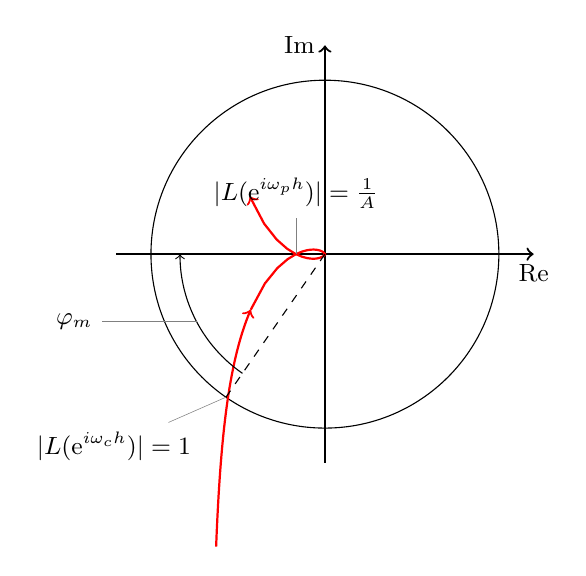
\begin{tikzpicture}[node distance=4cm]

\def\minomega{0.18}
\pgfmathsetmacro{\startangle}{ -90*sign(-\minomega) -2*atan(-\minomega/1) }
\pgfmathsetmacro{\endangle}{ -90*sign(\minomega) -2*atan(\minomega/1) }
\pgfmathsetmacro{\omegac}{0.2950}
%\pgfmathsetmacro{\gainatomegac}{1/(abs(\omegac)*(\omegac*\omegac+1))} % Should be 3
\pgfmathsetmacro{\gainatomegac}{3}
\pgfmathsetmacro{\angleatomegac}{-90*sign(\omegac) -2*atan(\omegac)-1.8}
%\pgfmathsetmacro{\pindist}{ 1/(abs(\pinomega)*(\pinomega*\pinomega + 1))} 
\begin{polaraxis}[
   xshift=0cm,
   width=6cm,
   height=6cm,
   clip=false,
   xtick=\empty,
   ytick=\empty,
   ymin=0, ymax=3,
   y tick label style={anchor=north east},
]
\draw[->, thick] (axis cs: 270, 3.6) -- (axis cs: 90, 3.6) node [left] {\small $\mathrm{Im}$};
\draw[->, thick] (axis cs: 180, 3.6) -- (axis cs: 0, 3.6) node [below] {\small $\mathrm{Re}$};
\addplot+[->,thick, red, no markers, domain=-100:-0.5, samples=800] ( {-90*sign(x) -2*atan(x/1)}, {1/(abs(x)*(x*x+1))}); 
%\addplot+[->,thick, red, no markers, domain=-0.5:-\minomega, samples=100] ( -90*sign(x) -2*atan(x/1), 1/(abs(x)*(x*x+1))); 
\addplot+[->,thick, red, no markers, domain=\minomega:0.5, samples=100] ( {-90*sign(x) -2*atan(x/1)}, {1/(abs(x)*(x*x+1))}); 
\addplot+[thick, red, no markers, domain=0.5:100, samples=800] ( {-90*sign(x) -2*atan(x/1)}, {1/(abs(x)*(x*x+1))}); 
%\addplot+[->,thin, red, no markers, dashed, domain=\startangle:45, samples=400] (x, 1/(abs(-\minomega)*(\minomega*\minomega+1))); %
%
%\addplot+[->,thin, red, no markers, dashed, domain=45:-45, samples=400] (x, 1/(abs(-\minomega)*(\minomega*\minomega+1))); %
%\addplot+[->,thin, red, no markers, dashed, domain=-45:\endangle, samples=400] (x, 1/(abs(-\minomega)*(\minomega*\minomega+1)));
\addplot+[dashed, black, no markers] coordinates {(0,0)  (\angleatomegac,\gainatomegac)};
%\addplot+[dashed, black, no markers] coordinates {(0,0) (-110,3)};
\node[coordinate, pin=225:{\small $|L(\mathrm{e}^{i\omega_ch})|=1$}] at (axis cs: \angleatomegac, \gainatomegac) {}; 
\node[coordinate, pin=90:{\small$|L(\mathrm{e}^{i\omega_ph})|=\frac{1}{A}$}] at (axis cs: -180, 0.5) {}; 

\draw[thin, black, ->] (axis cs: \angleatomegac, 2.5) arc (\angleatomegac:-180:1.84cm) node[coordinate, pos=0.5] (arcmid) {};
\node[coordinate,  pin={[pin distance=1.2cm,] -180:{\small $\varphi_m$}}] at (arcmid) {}; 

\end{polaraxis}

\end{tikzpicture}
\end{document}
